% ***************************************************************************************
% ************************************* CAPÍTULO II *************************************
% ***************************************************************************************
\chapter{DESCRIPCIÓN FUNCIONAL}
\thispagestyle{empty}
Una vez conocidos los elementos que componen un BMS, así como los protocolos de comunicación utilizados para transmitir a los diferentes niveles de control; se puede comenzar a estudiar los diferentes sub-sistemas a implementar, para así definir los parámetros de diseño para las necesidades específicas del presente caso de estudio.

Para ello se estudian los tres sistemas que se desean implementar en
este trabajo: sistema de iluminación, sistema HVAC y sistema de bombeo variable. Además, previamente, se analizan lógicas utilizadas en estos sistemas para mejorarlas en la implementación. Por otro lado se detalla el funcionamiento de una interfaz gráfica para el manejo y supervisión de cada subsistema, a partir de los datos obtenidos de cada uno de ellos.

\section{Sistema de iluminación}
El sistema de regulación de iluminación se encarga de gestionar las luminarias de las zonas comunes. Para esto se implementan diferentes tipos de actuadores como: pulsadores, sensor de presencia, sensores de luminosidad. Dicho sistema se encarga de regular el ON/OFF de los circuitos de iluminación. Con lo cual contribuye considerablemente al ahorro y eficiencia energética del edificio.

\subsection{Condiciones de operación}
Por lo general las lógicas de este subsistema están centradas sobre uno de los
controladores principales a nivel de control, donde este puede
controlar las luminarias a través de sus salidas analógicas o con
ayuda de otros dispositivos como pulsadores o relés con sus respectivas salidas digitales. Para entender qué dispositivos son necesarios y que tipo de lógica se puede implementar, se estudian las lógicas previas empleadas en instalaciones anteriores.
\subsection{Lógicas previas}
Los diferentes tipos de instalaciones disponen por lo general de 4
lógicas, que permiten automatizar y contribuir con el ahorro y
eficiencia energética. Estas son:

\begin{itemize}
    \item \textbf{Encendido por horario:} 
se establece un horario para regular la
luminosidad del área correspondiente dependiendo de hora, día o fecha en específico. Por lo general esta lógica es utilizada para áreas como pasillos o habitaciones concurridas diariamente, con lo se puede administrar el uso de luminarias según el requerimiento de los usuarios para las diferentes áreas.

\item \textbf{Encendido por presencia:} 
se establece un sensor de presencia para
regular la luminosidad dependiendo del área y lo concurrido de esta.
Por lo general, esta estrategia se utiliza para áreas poco
concurridas o donde su uso no tiene un patrón definido. Por lo cual el
sensor de presencia contribuye de manera eficiente en el uso del
recurso lumínico.

\item \textbf{Encendido por tiempo:}
se establece un pulsador en áreas estratégicas del área correspondiente, con una cantidad de tiempo determinado. Con esto los usuarios pueden encender las distintas luminarias, sin la preocupación de olvidar el apagado de estas posteriormente. Normalmente, este tipo de lógicas se utilizan en complemento con las dos anteriores para permitirle al usuario extender o ajustar de mejor manera la regulación a su necesidad

\item \textbf{Encendido por manejo de luz:}
se utilizan sensores fotovoltaicos en
las diferentes áreas a controlar. Los sensores se encargan de
detectar la incidencia de luz natural en el espacio, y pueden tanto
encender como graduar la intensidad de las luminarias.
\end{itemize}
\section{Sistema HVAC}
Un Sistema de Calefacción, Ventilación y Aire Acondicionado (HVAC,
\textit{Heating Ventilation and Air Conditioning} por sus siglas en inglés) está diseñado para mantener las condiciones de confort térmico necesarias para el proceso de fabricación de un
determinado producto, o bien, las condiciones óptimas para una necesidad en específico. Para ello se realiza el acondicionamiento del aire, este acondicionamiento consiste en el proceso de limpiar y hacer circular aire dentro del espacio, controlando, además, su temperatura y contenido de humedad.

La correcta aplicación de control sobre este sistema se basa en los
principios de reducción de ganancia de calor interior y de
ventilación, por lo cual, se disminuyen los requerimientos de
refrigeración mecánica para lograr las condiciones de confort. Esto se
refleja en una reducción del consumo de energía, y de costos de
funcionamiento, lo cual representa una importante suma de ahorro de energía por parte de los usuarios.

Los sistemas de refrigeración se caracterizan por la presencia de un compendio de componentes, que se encargan de cumplir la tarea del proceso de extracción de calor; dichos componentes son: compresor, condensador y evaporador. Según el tipo de requerimiento, se elige la clase de sistema de condensación necesaria para cumplir con dichas necesidades. Es por ello que se dividen principalmente en dos tipos de sistemas:
\begin{itemize}
    \item \textbf{Sistemas de expansión directa:}
equipos autónomos, diseñados para utilizar refrigerante como medio de enfriamiento del aire. Siendo los condensadores del equipo de refrigeración enfriados por aire, por lo tanto poseen su propio ciclo de refrigeración y no dependen de un equipo central. Estos a su vez, se dividen en dos: equipos compactos y equipos divididos.

\item \textbf{Sistemas centrales:}
son aquellos sistemas que centralizan la
generación de fluido térmico, encargado de transportar la energía a los locales a acondicionar. Siendo los condensadores del equipo de
refrigeración enfriado con ayuda de dicho fluido térmico proveniente
del sistema central. Este sistema se divide a su vez en sistemas: todo aire, aire-agua, todo agua.
\end{itemize}

Para el presente proyecto se utilizó un sistema de expansión directa de equipos divididos, el cual se explica a continuación. Sin embargo
para el sistema de bombeo variable es necesario conocer el
funcionamiento de un sistema central  aire-agua , para el diseño de la
lógica de control pertinente. Este sistema es explicado en el punto (falta especificar punto de sistema aire agua).

\subsection{Condiciones de operación}
Los equipos divididos están compuestos por dos unidades separadas. Una unidad exterior compuesta por un compresor y condensador, y, la unidad interior compuesta por un evaporador, ambas unidas por tuberías por donde circula refrigerante. Ver figura \ref{fig:sistemaenestudio}

\begin{figure}[H]
    \centering
    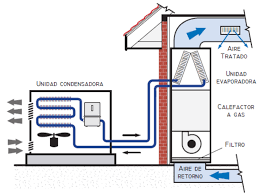
\includegraphics[width=0.60\textwidth]{2_MainMatter/Capitulo2/Imagenes/sistemaenestudio.PNG}
    \caption{Sistema de equipos divididos\cite{Sistemadividido}}
    \label{fig:sistemaenestudio}
\end{figure}

Todo el aire de retorno pasa por la unidad de tratamiento central, por
lo que sufre una nueva filtración y corrección de la humedad, lo que
permite un incremento en la buena calidad del aire. Por otro lado el aire de renovación es captado por una única toma exterior, lo que permite una mejor ubicación de la misma, lo que proporciona ahorro en espacio y menor incidencia de ruido sobre los usuarios.

Este sistema permite la posibilidad de utilizar elementos de control
de las condiciones ambientales de cada local. Uno de ellos es el
damper o válvulas que controlan el flujo del aire en todo el sistema
de ductos en el espacio (Ver figura \ref{fig:ejemplodamper}), lo que permite adaptar temperaturas por cargas térmicas en zonas determinadas.

\begin{figure}[H]
    \centering
    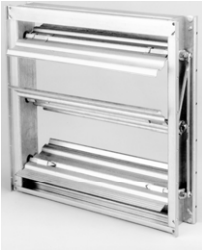
\includegraphics[width=0.30\textwidth]{2_MainMatter/Capitulo2/Imagenes/ejemplodamper.PNG}
    \caption{Balancing Damper\cite{Dampers}}
    \label{fig:ejemplodamper}
\end{figure}

\subsection{Lógicas previas}
Los diferentes tipos de instalaciones que disponen la
implementación de equipos divididos con dampers/válvulas de control de flujo de aire, utilizan por lo general de 3 lógicas, que permiten
automatizar y contribuir con el ahorro y eficiencia energética. Estas
son:
\begin{itemize}
    \item \textbf{Control por horario:}
se establece un horario para regular la temperatura del área correspondiente dependiendo, como en el caso del sistema lumínico, de hora, dia o fecha en específico. Por lo general esta lógica es utilizada para controlar la temperatura de áreas durante días en específico, aumentando la temperatura requerida en la \textit{Unidad Manejadora de Aire} (UMA), lo que requiere un menor uso del compresor, y, en consecuencia, un ahorro energético.

 \item \textbf{Control por presencia:}
se establece un sensor de presencia para regular la temperatura dependiendo del área y su afluencia. Al igual que en el sistema lumínico, esta estrategia se utiliza para áreas poco concurridas o donde su uso puede tener un patrón definido. Por lo cual se puede aumentar la temperatura en dichas áreas, sin perjudicar el confort térmico de los usuarios, ahorrando energía eficientemente.

 \item \textbf{Control por requerimiento:}
se establece un controlador en áreas estratégicas del área pertinente, con la capacidad de indicarle a la UMA correspondiente, la necesidad térmica adecuada. De este  modo, los usuarios pueden ajustar la temperatura del área en uso, según sus gustos particulares. Normalmente este tipo de lógicas se utilizan en complemento con las dos anteriores para permitirle al usuario extender o ajustar de mejor manera la regulación a su perfil.  
\end{itemize}
\section{Sistema de bombeo primario variable}
El sistema de bombeo primario variable, es un elemento que forma parte de un sistema central de HVAC. Este puede ser utilizado tanto para sistemas aire-agua, como para sistemas todo agua. Ambos tienen en común la presencia de un sistema centralizado de enfriamiento, las cuales generan enfriamiento en un solo lugar para su distribución a múltiples ubicaciones en el área que se desea cubrir. El sistema de enfriamiento se utiliza en casi toda clase de edificios, sin embargo son de mayor eficiencia para edificaciones y complejos de gran tamaño donde existe una alta densidad de demanda energética.

En este trabajo se estudiará el sistema de agua helada con planta de enfriamiento para el uso de sistemas de bombeo variable. Es por ello que, para un mejor entendimiento de las lógicas a aplicar, se estudia en el próximo punto el sistema tipo aire-agua.

\subsection{Sistema central aire-agua}
Se basa en la distribución de energía a los diversos locales a través de circuitos de agua enfriada y aire. Estos sistemas se componen de:
\begin{itemize}
 \item \textbf{Enfriadores de agua:}
 equipos frigoríficos que utilizan el ciclo de refrigeración para enfriar agua. En este caso es el Chiller (ver figura \ref{fig:ejemploChiller}), el cual contiene los mismos componentes, evaporador, compresor, condensador y  válvula de expansión.
 
 \begin{figure}[H]
    \centering
    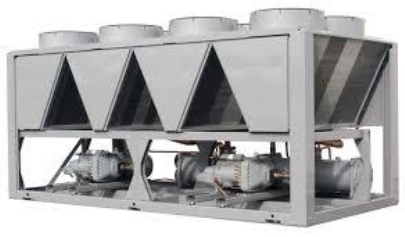
\includegraphics[width=0.40\textwidth]{2_MainMatter/Capitulo2/Imagenes/Chiller.PNG}
    \caption{Ejemplo de Chiller\cite{Sistemadividido}}
    \label{fig:ejemploChiller}
\end{figure}

 \item \textbf{Manejadores de aire:}
  son equipos compuestos por un intercambiador de calor agua-aire, un ventilador, filtros de aire, una bandeja de drenaje y un gabinete aislado térmicamente con una entrada de aire.
  
  Dentro de los tubos del intercambiador se hace circular agua helada o agua caliente, lográndose las funciones de calefacción o refrigeración. Normalmente el agua que se hace circular por los tubos del intercambiador proviene del chiller, y se llega a este gracias a bombas centrifugas.  En la figura \ref{fig:ejemploAire-Agua} se puede observar el esquema de una unidad central aire-agua con todos sus elementos.
  
   \begin{figure}[H]
    \centering
    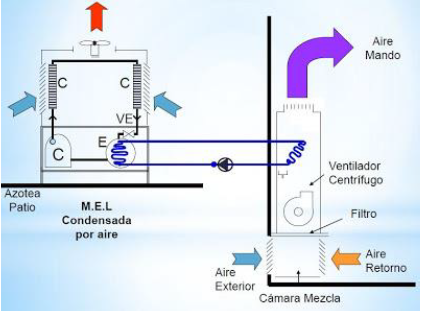
\includegraphics[width=0.60\textwidth]{2_MainMatter/Capitulo2/Imagenes/SistemaAguaAire.PNG}
    \caption{Sistema Central Aire-Agua \cite{Sistemadividido}}
    \label{fig:ejemploAire-Agua}
\end{figure}

\end{itemize}

Este tipo de sistemas permite individualidad entre los diferentes ambientes o locales acondicionados, ya que cada localidad es servida por cada UMA, por lo que cada una de estas es acondicionada independientemente, por lo tanto el control de la temperatura y humedad corresponde a las condiciones particulares de cada espacio.

\subsection{Condiciones de operación}
La configuración de un sistema central se basa en el uso y la aplicación del mismo. El flujo variable primario envía este a través del enfriador (Chiller) y bombea directamente al punto de uso. Se puede lograr con válvulas de control automáticas bidireccionales en el equipo terminal y el variador de frecuencia (VFD \textit{Variable Frequency Drive} por sus siglas en inglés), bombeo o control de presión de distribución, además con una válvula de bypass se garantiza el mantenimiento de los caudales mínimos de los equipos en todo momento. En la figura \ref{fig:SistemaBombeoPrimario} se observa la disposición de un planta de agua helada.

 \begin{figure}[H]
    \centering
    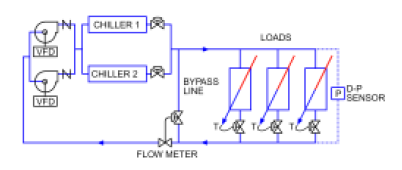
\includegraphics[width=0.70\textwidth]{2_MainMatter/Capitulo2/Imagenes/PlantaAguaHelada.PNG}
    \caption{Sistema de bombeo primario variable \cite{SistemaBombeoPrimario}}
    \label{fig:SistemaBombeoPrimario}
\end{figure}
Las condiciones de caudal y presión de distribución, están dadas por el punto de operación del sistema dependiendo del requerimiento en las cargas del edificio (Serpentines de UMAS). Es por ello que el control variable de este flujo representa un ahorro energético significativo en comparación con el flujo constante para la operación de la planta.

El funcionamiento de bombas centrífugas dependen de dos variables como lo son el diferencial de presión que existe entre entrada y salida de la bomba, y la capacidad de envío de flujo de la misma. Este tipo de bombas presenta la característica de tener la diferencia de presión creciente cuando el flujo de la bomba decrece. En la figura \ref{fig:CurvaControlTaco} se puede observar la curva característica de una bomba centrífuga.

\begin{figure}[H]
    \centering
    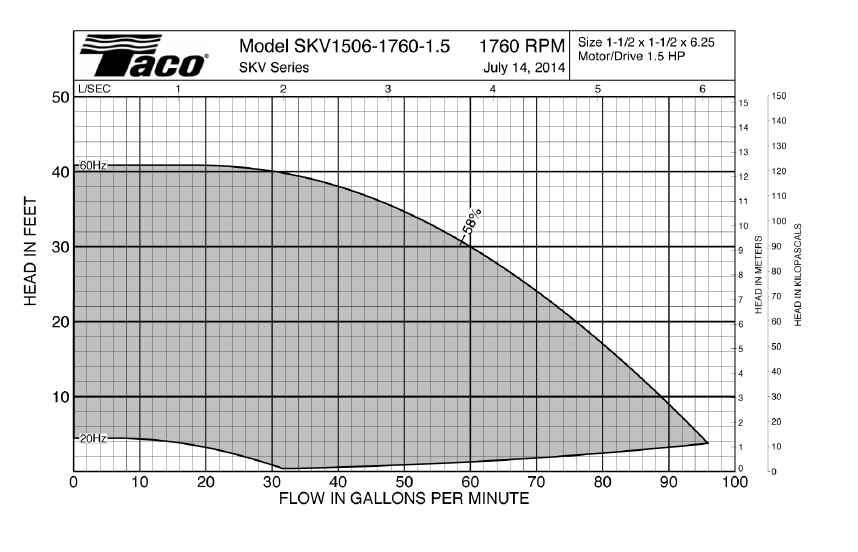
\includegraphics[width=0.80\textwidth]{2_MainMatter/Capitulo2/Imagenes/CurvacontrolTaco.PNG}
    \caption{Curvas bomba centrífuga Taco \cite{BombaTaco}}
    \label{fig:CurvaControlTaco}
\end{figure}

\subsection{Lógicas previas}

\begin{itemize}
 \item \textbf{Control por presión constante:}
 se basa en controlar el punto de operación de la bomba basado en una presión específica. En la figura \ref{fig:CurvaControlTacoP} se puede observar que siguiendo las características de una bomba centrífuga, al  mantener la presión, el flujo de esta varia.
 
 \begin{figure}[H]
    \centering
    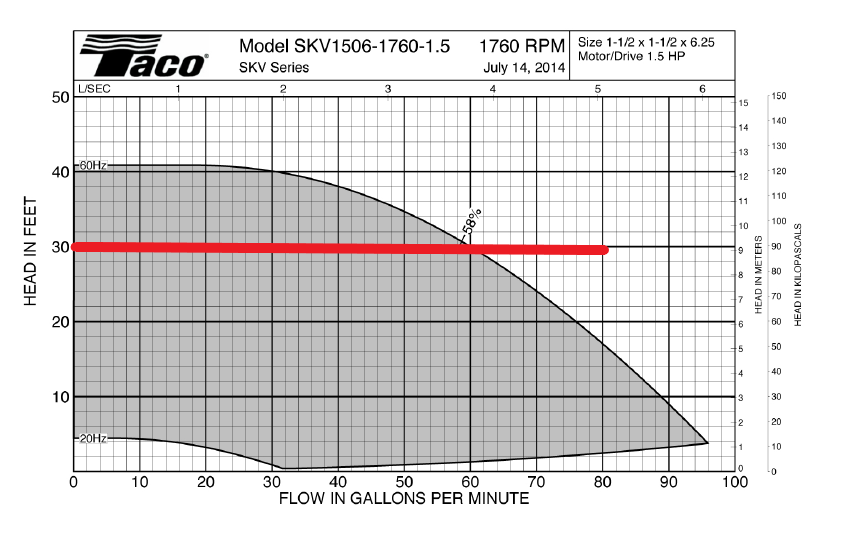
\includegraphics[width=0.80\textwidth]{2_MainMatter/Capitulo2/Imagenes/CurvacontrolTacoPconstante.png}
    \caption{Control por presión constante}
    \label{fig:CurvaControlTacoP}
\end{figure}

\item \textbf{Control por flujo constante:}
se basa en controlar el punto de operación de la bomba basado en un caudal en específico. En la figura \ref{fig:CurvaControlTacoQ} se puede observar que al mantener un caudal fijo, por características de las bombas, la presión aumenta o disminuye para satisfacer el caudal requerido.

 
 \begin{figure}[H]
    \centering
    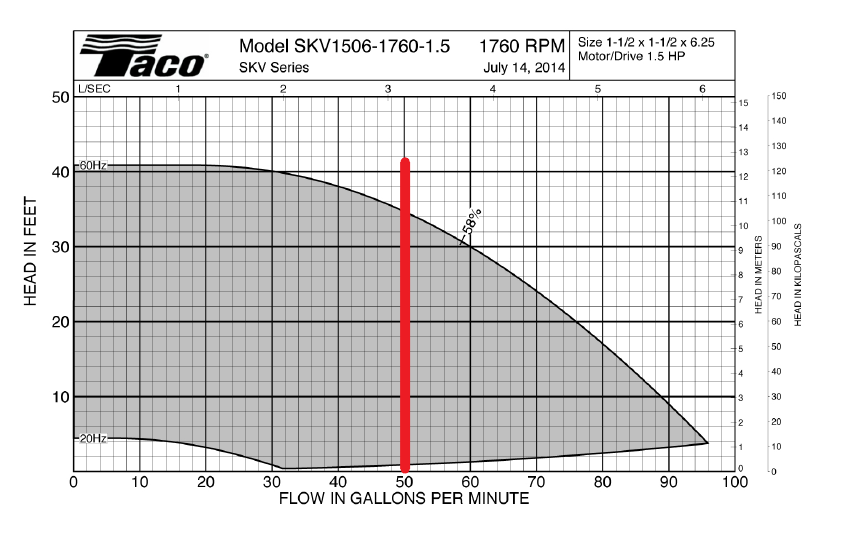
\includegraphics[width=0.80\textwidth]{2_MainMatter/Capitulo2/Imagenes/CurvacontrolTacoQconstante.png}
    \caption{Control por flujo constante}
    \label{fig:CurvaControlTacoQ}
\end{figure}

\item \textbf{Control por curva ajustada:}
se controla el punto de operación de la bomba, mediante una curva de control establecida por rendimiento y requerimientos. En la figura \ref{fig:CurvaControlTacoControl} se observa como este tipo de lógica permite satisfacer diferentes requerimientos de caudal, tratando de seguir la curva de eficiencia de la bomba. Lo que permite un uso
ajustado a las necesidades requeridas. 

\begin{figure}[H]
    \centering
    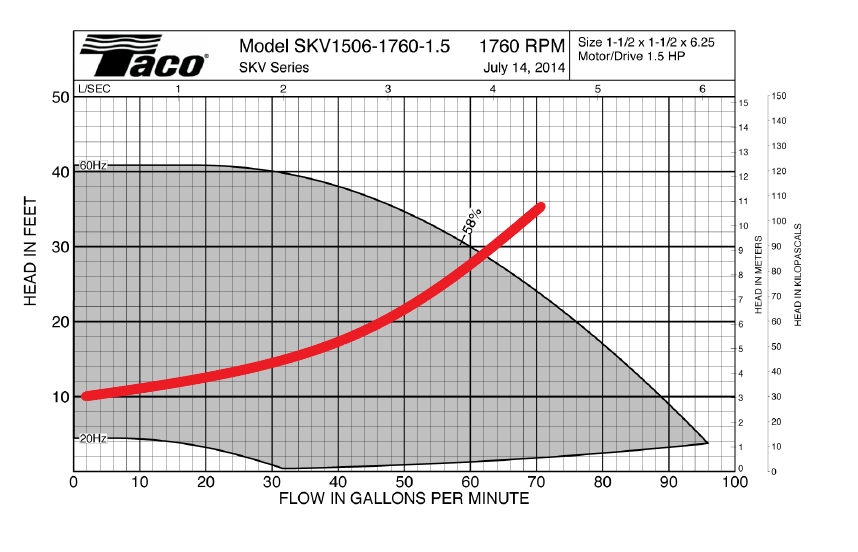
\includegraphics[width=0.80\textwidth]{2_MainMatter/Capitulo2/Imagenes/CurvacontrolTacoCurva.png}
    \caption{Control por curva ajustada}
    \label{fig:CurvaControlTacoControl}
\end{figure}

\end{itemize}

\section{Interfaz Gráfica}
\subsection{Lógicas previas}
\section{Estructura del espacio}
